% Testing the service
\section{Testing the Service}
\begin{frame}{Testing Considerations}
    The most commons development cases of Machine Learning services are those where the building of the model and the service are done completely separated and even by different teams.

    That implies we aren't in control of the training process so that we cannot test the model until both are merged.
\end{frame}

\begin{frame}{Validation vs Verification}
    \rowcolors{1}{}{gray!20}
    \begin{tabular}{lp{1.6in}p{1.6in}}
        \toprule
        \textbf{Criteria} & \textbf{Verification} & \textbf{Validation} \\
        \midrule
        \emph{Definition} & The process of evaluating products of a development phase to determine whether they meet the specified requirements. & The process of evaluating software during or at the end of the development process to determine whether it satisfies specified business requirements. \\
        \emph{Objective} & To ensure that the product is being built according to the requirements and design specifications. & To demonstrate that the product fulfills its intended use when placed in its intended environment. \\
        \emph{Question} & Are we building the product right? & Are we building the right product? \\
        \bottomrule
    \end{tabular}
\end{frame}

\begin{frame}[fragile]{Test Specification: Verification}
    \footnotesize{
        \begin{verbatim}
## Endpoint Verification
Tags: functional, verification

Verify if the endpoint that allows interaction with Sentiment Analyzer
is properly defined based on specifications. It must provide a query
parameter **text** that acts as the input of the model and it cannot be
empty. The response must be a JSON containing three attributes:
**text**, **score** and **sentiment**.

* Request sentiment analysis with text "Perdy is testing this" returns "200"
* Response schema contains attributes
    |Attribute|
    |---------|
    |text     |
    |score    |
    |sentiment|
* Request sentiment analysis with text "" returns "400"
        \end{verbatim}
    }
\end{frame}

\begin{frame}[fragile]{Test Specification: Validation}
    \footnotesize{
        \begin{verbatim}
## Model Validation
Tags: ml, validation

Validate the model predictions against a set of fixed data. This data set
must contains a minimum list of well-known pairs of input and output to
check that after retraining the model it will continue behaving the same
way against these inputs.

* Analyze and validate the following texts <table:data/sentiment_analysis.csv>
        \end{verbatim}
    }
\end{frame}

\begin{frame}[fragile]{Step Implementation}
    \begin{minted}[fontsize=\footnotesize]{python}
@step("Response schema contains attributes <table>")
def assert_response_schema(table):
    response = data_store.scenario["response"]

    for attribute in table.get_column_values_with_name("Attribute"):
        assert attribute in response
    \end{minted}
\end{frame}

\begin{frame}{Console Output}
    \begin{figure}
        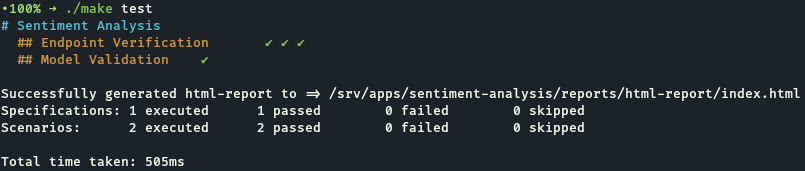
\includegraphics[width=\textwidth]{img/test-console-output.png}
    \end{figure}
\end{frame}

\begin{frame}{HTML Output}
    \begin{figure}
        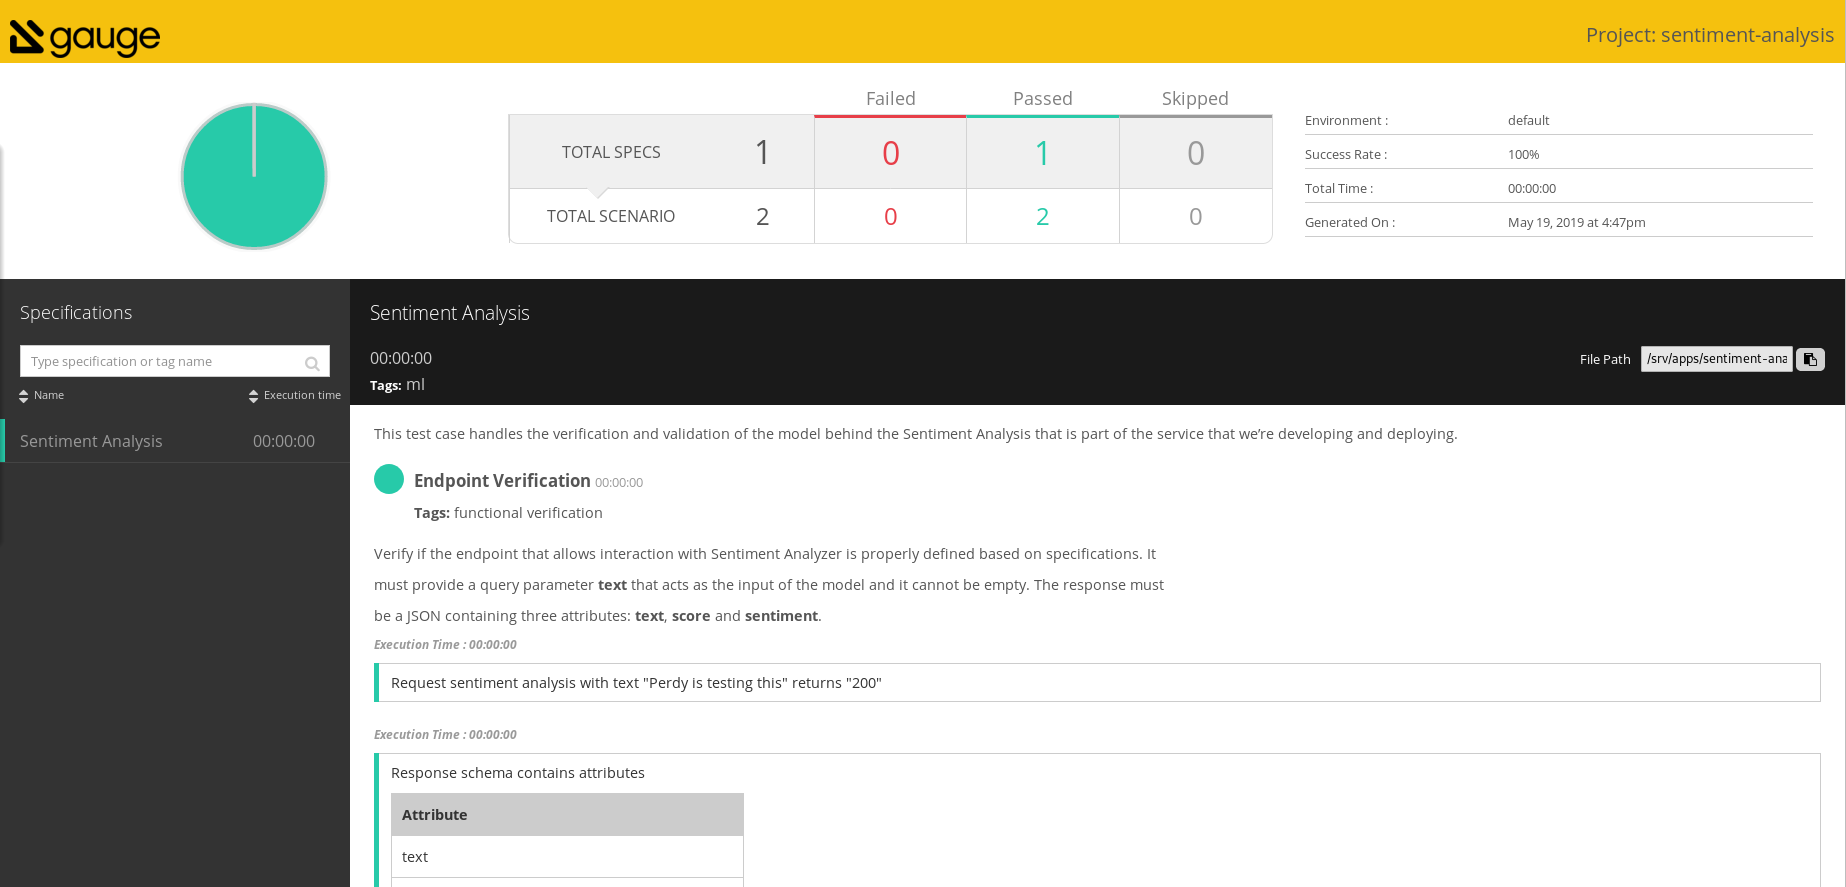
\includegraphics[width=\textwidth]{img/test-html-output.png}
    \end{figure}
\end{frame}
